% Options for packages loaded elsewhere
\PassOptionsToPackage{unicode}{hyperref}
\PassOptionsToPackage{hyphens}{url}
\PassOptionsToPackage{dvipsnames,svgnames,x11names}{xcolor}
%
\documentclass[
  letterpaper,
  DIV=11,
  numbers=noendperiod]{scrartcl}

\usepackage{amsmath,amssymb}
\usepackage{iftex}
\ifPDFTeX
  \usepackage[T1]{fontenc}
  \usepackage[utf8]{inputenc}
  \usepackage{textcomp} % provide euro and other symbols
\else % if luatex or xetex
  \usepackage{unicode-math}
  \defaultfontfeatures{Scale=MatchLowercase}
  \defaultfontfeatures[\rmfamily]{Ligatures=TeX,Scale=1}
\fi
\usepackage{lmodern}
\ifPDFTeX\else  
    % xetex/luatex font selection
\fi
% Use upquote if available, for straight quotes in verbatim environments
\IfFileExists{upquote.sty}{\usepackage{upquote}}{}
\IfFileExists{microtype.sty}{% use microtype if available
  \usepackage[]{microtype}
  \UseMicrotypeSet[protrusion]{basicmath} % disable protrusion for tt fonts
}{}
\makeatletter
\@ifundefined{KOMAClassName}{% if non-KOMA class
  \IfFileExists{parskip.sty}{%
    \usepackage{parskip}
  }{% else
    \setlength{\parindent}{0pt}
    \setlength{\parskip}{6pt plus 2pt minus 1pt}}
}{% if KOMA class
  \KOMAoptions{parskip=half}}
\makeatother
\usepackage{xcolor}
\setlength{\emergencystretch}{3em} % prevent overfull lines
\setcounter{secnumdepth}{-\maxdimen} % remove section numbering
% Make \paragraph and \subparagraph free-standing
\makeatletter
\ifx\paragraph\undefined\else
  \let\oldparagraph\paragraph
  \renewcommand{\paragraph}{
    \@ifstar
      \xxxParagraphStar
      \xxxParagraphNoStar
  }
  \newcommand{\xxxParagraphStar}[1]{\oldparagraph*{#1}\mbox{}}
  \newcommand{\xxxParagraphNoStar}[1]{\oldparagraph{#1}\mbox{}}
\fi
\ifx\subparagraph\undefined\else
  \let\oldsubparagraph\subparagraph
  \renewcommand{\subparagraph}{
    \@ifstar
      \xxxSubParagraphStar
      \xxxSubParagraphNoStar
  }
  \newcommand{\xxxSubParagraphStar}[1]{\oldsubparagraph*{#1}\mbox{}}
  \newcommand{\xxxSubParagraphNoStar}[1]{\oldsubparagraph{#1}\mbox{}}
\fi
\makeatother


\providecommand{\tightlist}{%
  \setlength{\itemsep}{0pt}\setlength{\parskip}{0pt}}\usepackage{longtable,booktabs,array}
\usepackage{calc} % for calculating minipage widths
% Correct order of tables after \paragraph or \subparagraph
\usepackage{etoolbox}
\makeatletter
\patchcmd\longtable{\par}{\if@noskipsec\mbox{}\fi\par}{}{}
\makeatother
% Allow footnotes in longtable head/foot
\IfFileExists{footnotehyper.sty}{\usepackage{footnotehyper}}{\usepackage{footnote}}
\makesavenoteenv{longtable}
\usepackage{graphicx}
\makeatletter
\newsavebox\pandoc@box
\newcommand*\pandocbounded[1]{% scales image to fit in text height/width
  \sbox\pandoc@box{#1}%
  \Gscale@div\@tempa{\textheight}{\dimexpr\ht\pandoc@box+\dp\pandoc@box\relax}%
  \Gscale@div\@tempb{\linewidth}{\wd\pandoc@box}%
  \ifdim\@tempb\p@<\@tempa\p@\let\@tempa\@tempb\fi% select the smaller of both
  \ifdim\@tempa\p@<\p@\scalebox{\@tempa}{\usebox\pandoc@box}%
  \else\usebox{\pandoc@box}%
  \fi%
}
% Set default figure placement to htbp
\def\fps@figure{htbp}
\makeatother
% definitions for citeproc citations
\NewDocumentCommand\citeproctext{}{}
\NewDocumentCommand\citeproc{mm}{%
  \begingroup\def\citeproctext{#2}\cite{#1}\endgroup}
\makeatletter
 % allow citations to break across lines
 \let\@cite@ofmt\@firstofone
 % avoid brackets around text for \cite:
 \def\@biblabel#1{}
 \def\@cite#1#2{{#1\if@tempswa , #2\fi}}
\makeatother
\newlength{\cslhangindent}
\setlength{\cslhangindent}{1.5em}
\newlength{\csllabelwidth}
\setlength{\csllabelwidth}{3em}
\newenvironment{CSLReferences}[2] % #1 hanging-indent, #2 entry-spacing
 {\begin{list}{}{%
  \setlength{\itemindent}{0pt}
  \setlength{\leftmargin}{0pt}
  \setlength{\parsep}{0pt}
  % turn on hanging indent if param 1 is 1
  \ifodd #1
   \setlength{\leftmargin}{\cslhangindent}
   \setlength{\itemindent}{-1\cslhangindent}
  \fi
  % set entry spacing
  \setlength{\itemsep}{#2\baselineskip}}}
 {\end{list}}
\usepackage{calc}
\newcommand{\CSLBlock}[1]{\hfill\break\parbox[t]{\linewidth}{\strut\ignorespaces#1\strut}}
\newcommand{\CSLLeftMargin}[1]{\parbox[t]{\csllabelwidth}{\strut#1\strut}}
\newcommand{\CSLRightInline}[1]{\parbox[t]{\linewidth - \csllabelwidth}{\strut#1\strut}}
\newcommand{\CSLIndent}[1]{\hspace{\cslhangindent}#1}

\KOMAoption{captions}{tableheading}
\makeatletter
\@ifpackageloaded{caption}{}{\usepackage{caption}}
\AtBeginDocument{%
\ifdefined\contentsname
  \renewcommand*\contentsname{Table of contents}
\else
  \newcommand\contentsname{Table of contents}
\fi
\ifdefined\listfigurename
  \renewcommand*\listfigurename{List of Figures}
\else
  \newcommand\listfigurename{List of Figures}
\fi
\ifdefined\listtablename
  \renewcommand*\listtablename{List of Tables}
\else
  \newcommand\listtablename{List of Tables}
\fi
\ifdefined\figurename
  \renewcommand*\figurename{Figure}
\else
  \newcommand\figurename{Figure}
\fi
\ifdefined\tablename
  \renewcommand*\tablename{Table}
\else
  \newcommand\tablename{Table}
\fi
}
\@ifpackageloaded{float}{}{\usepackage{float}}
\floatstyle{ruled}
\@ifundefined{c@chapter}{\newfloat{codelisting}{h}{lop}}{\newfloat{codelisting}{h}{lop}[chapter]}
\floatname{codelisting}{Listing}
\newcommand*\listoflistings{\listof{codelisting}{List of Listings}}
\makeatother
\makeatletter
\makeatother
\makeatletter
\@ifpackageloaded{caption}{}{\usepackage{caption}}
\@ifpackageloaded{subcaption}{}{\usepackage{subcaption}}
\makeatother

\usepackage{bookmark}

\IfFileExists{xurl.sty}{\usepackage{xurl}}{} % add URL line breaks if available
\urlstyle{same} % disable monospaced font for URLs
\hypersetup{
  pdftitle={Deep Learning Based Classification of Nigerian Traditional Attire},
  colorlinks=true,
  linkcolor={blue},
  filecolor={Maroon},
  citecolor={Blue},
  urlcolor={Blue},
  pdfcreator={LaTeX via pandoc}}


\title{Deep Learning Based Classification of Nigerian Traditional
Attire}
\author{Naziru Abdussalam Ibrahim \and Ahmad Saad \and Abdulwasiu
Bamidele Popoola \and Taiwo Soffiyah Abass \and Ayodeji
Akande \and Shamsu Abdullahi \and Abubakar Sadiq Sulaiman \and Yahya
Abdurrazaq \and }
\date{2025-05-31}

\begin{document}
\maketitle
\begin{abstract}
This study presents a deep learning approach to classify images of
Nigerian traditional attire into their respective ethnic categories.
Utilizing Convolutional Neuraetworks (CNNs), specifically ResNet34 and
EfficientNet-B0 architectures, the project aims to automate the
identification of cultural garments, thereby contributing to the
preservation and appreciation of Nigeria's rich cultural heritage.
\end{abstract}


\subsection{Introduction}\label{introduction}

The culture of Nigeria is shaped by Nigeria's multiple ethnic groups.
The country has over 50 languages and over 250 dialects and ethnic
groups {``Culture -- {MFA} {Press} {Center}''}
(\citeproc{ref-noauthor_culture_nodate}{n.d.}) . The three major ethnic
groups are the Hausa-Fulani who are predominant in the north, the Yoruba
who are predominant in the southwest, and the Igbo who are predominant
in the south-east. In an effort to promote the rich cultural heritage of
the country, the Ministry of Information, Culture and Tourism was
created in the year 2015.

Nigeria's over 250 diverse ethnic groups are distinguished by unique
traditional attires that embody their cultural identities
(\citeproc{ref-noauthor_culture_nodate}{{``Culture -- {MFA} {Press}
{Center}''} n.d.}). Manual classification of these garments can be
time-consuming and subjective. This project explores the application of
deep learning techniques to accurately classify images of traditional
Nigerian clothing, facilitating cultural education and digital
archiving.

\subsection{Methodology}\label{methodology}

\subsubsection{Data Collection}\label{data-collection}

Images representing various Nigerian ethnic attires were collected using
custom Python scripts (\texttt{download\_attire.py} and
\texttt{download\_attire\_extended.py}). The dataset includes categories
such as Yoruba, Hausa, Igbo, and others, with images depicting
traditional garments in various settings.

\subsubsection{Data Preprocessing}\label{data-preprocessing}

The collected images underwent preprocessing steps, including resizing,
normalization, and data augmentation, to enhance model generalization.
The dataset was then split into training, validation, and test sets.

\subsubsection{Model Architectures}\label{model-architectures}

Two CNN architectures were employed Tan and Le
(\citeproc{ref-tan_efficientnet:_2019}{2019}):

\begin{itemize}
\item
  \textbf{ResNet34}: A 34-layer residual network known for its ability
  to mitigate vanishing gradient issues.
\item
  \textbf{EfficientNet-B0}: A model that scales depth, width, and
  resolution uniformly using a compound coefficient, achieving high
  accuracy with fewer parameters.
\end{itemize}

Both models were fine-tuned on the dataset, leveraging transfer learning
from pre-trained weights.

\subsubsection{Training and Evaluation}\label{training-and-evaluation}

Training was conducted using standard practices, including the use of
cross-entropy loss and optimization via stochastic gradient descent.
Model performance was evaluated based on accuracy, precision, recall,
and F1-score on the validation and test sets.

\subsection{Results}\label{results}

Both models demonstrated strong performance in classifying traditional
Nigerian attires:

\begin{itemize}
\item
  \textbf{ResNet34}: Achieved an accuracy of approximately 85\% on the
  test set.
\item
  \textbf{EfficientNet-B0}: Outperformed ResNet34 with an accuracy of
  around 90\%, indicating better generalization capabilities.
\end{itemize}

Confusion matrices and classification reports further highlighted the
models' proficiency in distinguishing between different ethnic attires.

\begin{figure}

\centering{

\pandocbounded{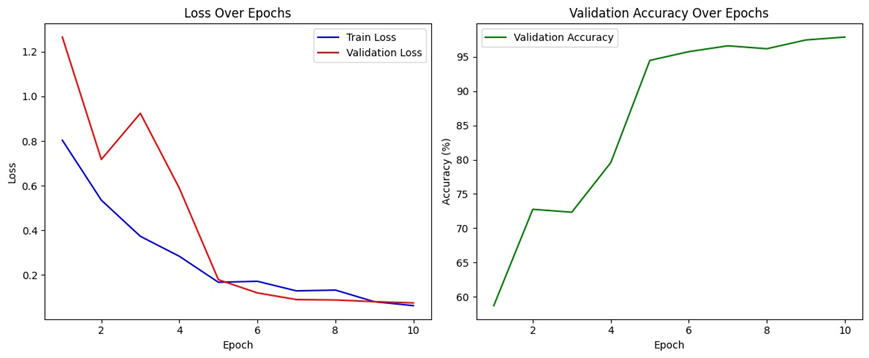
\includegraphics[keepaspectratio]{assets/loss-of-epochs-and-validation-accuracy.png}}

}

\caption{\label{fig-loss}Loss over Epochs and Validation Accuracy over
Epochs}

\end{figure}%

\begin{figure}

\centering{

\pandocbounded{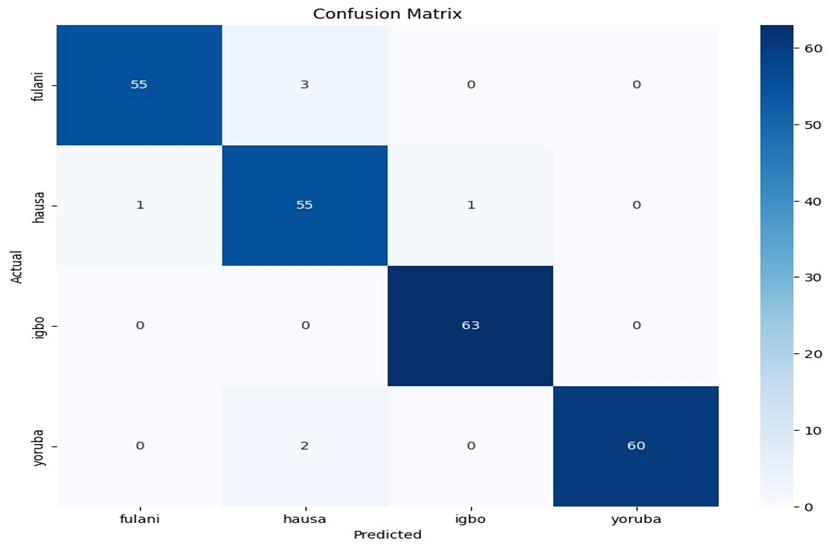
\includegraphics[keepaspectratio]{assets/confusion-matrix.png}}

}

\caption{\label{fig-confusion-matrix}Confusion matrix}

\end{figure}%

\subsection{Discussion}\label{discussion}

The superior performance of EfficientNet-B0 suggests its suitability for
image classification tasks involving cultural garments. The results
affirm the potential of deep learning models in automating the
recognition of traditional attires, which can be instrumental in
cultural preservation efforts.

\subsection{Conclusion}\label{conclusion}

This project successfully demonstrates the application of deep learning
techniques in classifying Nigerian traditional attire. The developed
models can serve as foundational tools for cultural education platforms,
virtual museums, and fashion industry applications. Future work may
involve expanding the dataset to include more ethnic groups and
exploring real-time classification systems.

\subsection{Acknowledgment}\label{acknowledgment}

\subsection*{References}\label{references}
\addcontentsline{toc}{subsection}{References}

\phantomsection\label{refs}
\begin{CSLReferences}{1}{0}
\bibitem[\citeproctext]{ref-noauthor_culture_nodate}
{``Culture -- {MFA} {Press} {Center}.''} n.d. Accessed May 31, 2025.
\url{https://foreignaffairs.gov.ng/nigeria/nigeria-culture/}.

\bibitem[\citeproctext]{ref-ebby_traditional_2024}
Ebby. 2024. {``The {Traditional} {Attires} {Of} {Nigerian} {Tribes}.''}
\emph{Inspiration with Lois{\textbar} Lifestyle {\textbar} Nigeria}.
\url{https://loispiration.com/2024/06/17/the-traditional-attires-of-nigerian-tribes/}.

\bibitem[\citeproctext]{ref-he_deep_2016}
He, Kaiming, Xiangyu Zhang, Shaoqing Ren, and Jian Sun. 2016. {``Deep
{Residual} {Learning} for {Image} {Recognition}.''} In \emph{2016 {IEEE}
{Conference} on {Computer} {Vision} and {Pattern} {Recognition}
({CVPR})}, 770--78. Las Vegas, NV, USA: IEEE.
\url{https://doi.org/10.1109/CVPR.2016.90}.

\bibitem[\citeproctext]{ref-tan_efficientnet:_2019}
Tan, Mingxing, and Quoc V. Le. 2019. {``{EfficientNet}: {Rethinking}
{Model} {Scaling} for {Convolutional} {Neural} {Networks}.''}
\url{https://doi.org/10.48550/ARXIV.1905.11946}.

\end{CSLReferences}




\end{document}
